\blindtext

\section{Reference Model}

\begin{figure}
    \centering
    \begin{subfigure}[t]{0.3\textwidth}
        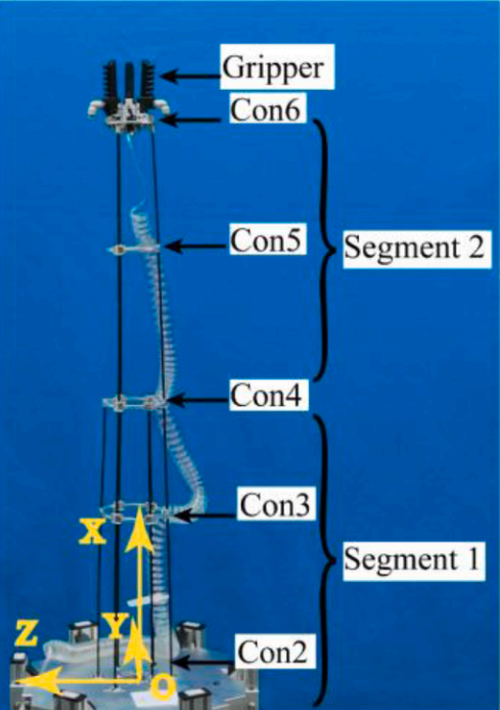
\includegraphics[width=\textwidth]{ref_robot}
        \caption{Sections and structure}
        \label{fig:ref_robot_structure}
    \end{subfigure}
    \begin{subfigure}[t]{0.3\textwidth}
        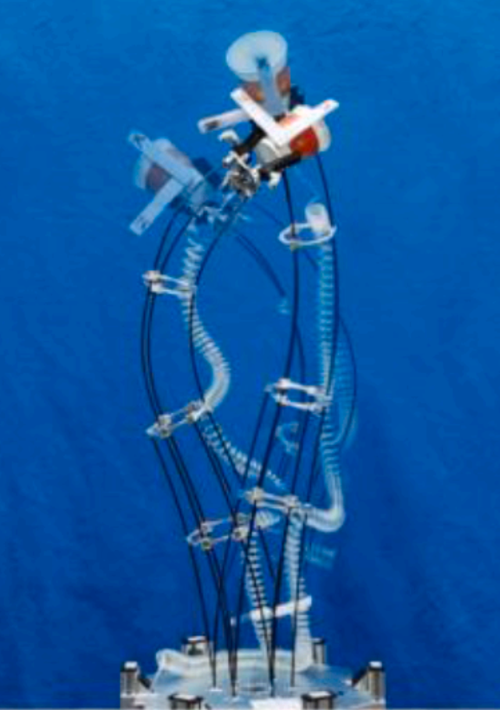
\includegraphics[width=\textwidth]{ref_robot_poses}
        \caption{Some end poses}
        \label{fig:ref_robot_poses}
    \end{subfigure}
    \caption{Reference robot structure}
    \caption*{Source: Adapted from \cite{wu2022}}
    \label{fig:ref_robot}
\end{figure}

\blindtext

\begin{figure}
    \centering
    \begin{subfigure}[t]{0.257\textwidth}
        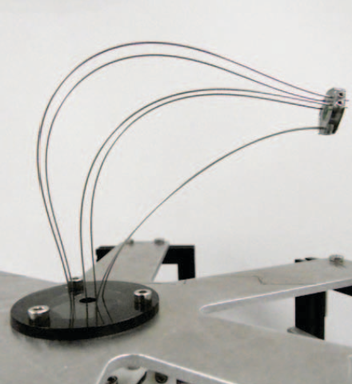
\includegraphics[width=\textwidth]{ref_robot2}
        \caption{No constraints}
        \label{fig:ref_robot2}
    \end{subfigure}
    \begin{subfigure}[t]{0.643\textwidth}
        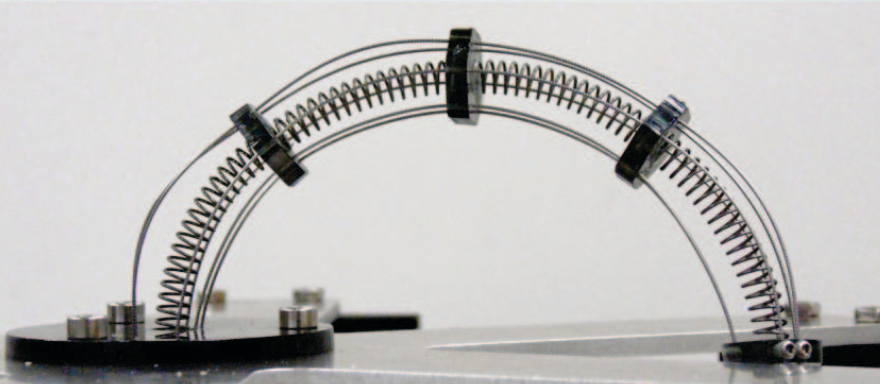
\includegraphics[width=\textwidth]{ref_robot2_cons}
        \caption{Extended range with intermediate constraints}
        \label{fig:ref_robot2_cons}
    \end{subfigure}
    \caption{Constraints and range of motion}
    \caption*{Source: Adapted from \cite{orekhov2017}}
    \label{fig:ref_robot2_constraints}
\end{figure}

\section{Rod Material}

\par [Rod definition]
\par [Table of materials]
\par [Table of properties of steel material]

\blindtext

\section{Design and Dimensions}

\blindtext

\section{Ring Constraints}

\blindtext
